\chapter[High Resolution Spectrometers (HRS)]{High Resolution Spectrometers (HRS)
\footnote{
  $CVS~revision~ $Id: hrs-1999.tex,v 1.7 2008/04/01 16:51:59 lerose Exp $ $ 
}
\footnote{Authors: J.LeRose \email{lerose@jlab.org}}
}
\label{chap:hrs}
\section{Overview}
   
The Hall A spectrometers and associated instrumentation are designed to 
perform high resolution and high accuracy experiments.  The goal is to 
achieve a missing mass resolution of $\sim$ 200-500 keV to clearly 
identify the nuclear final state.  An absolute accuracy of $\sim$ 1\% is 
also required by the physics program planned in the Hall, which implies 
$\sim$ 10$^{-4}$ accuracy in the determination of particle momenta and 
$\sim$ 0.1 mr in the knowledge of the scattering angle.

The instruments needed are a high resolution electron spectrometer 
(HRES) and a high resolution hadron spectrometer (HRHS), both with a 
large angular and momentum acceptance.

\begin{figure}[tbp]
\begin{center}
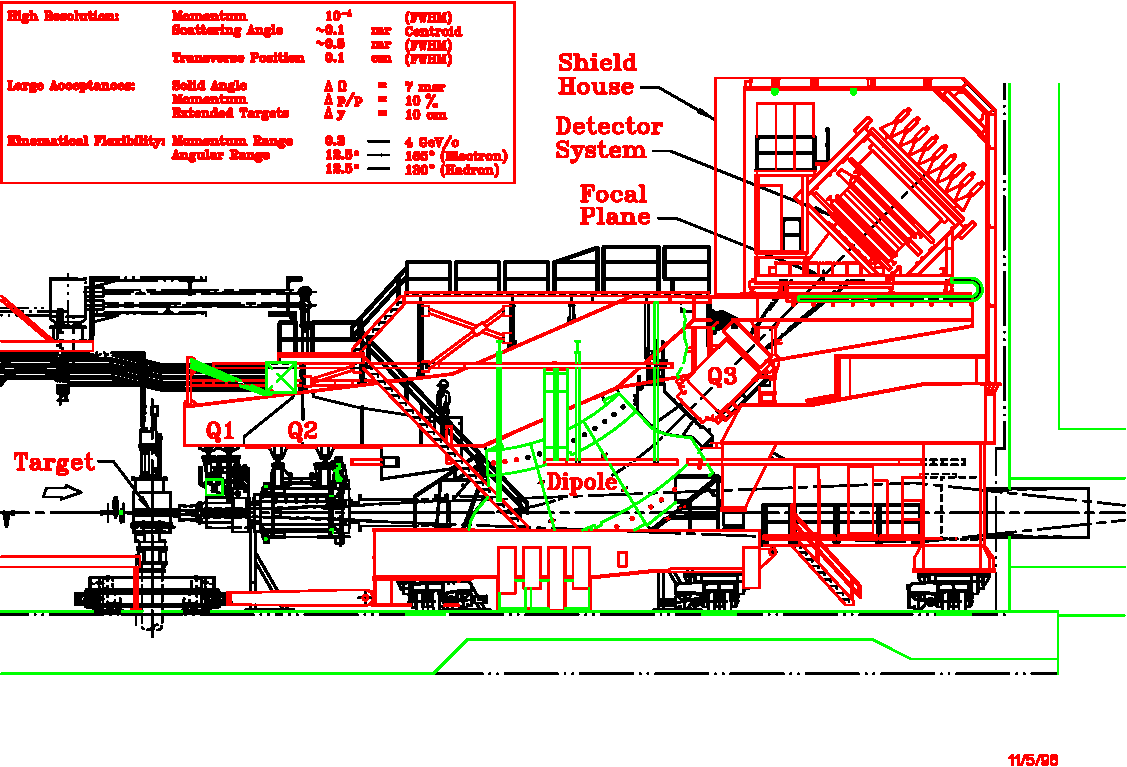
\includegraphics[angle=0,width=0.9\textwidth,clip]{figure0101_r}
\caption[Spectrometers: Elevation View of Hall~A HRS]{A side view of the Hall~A
HRS spectrometer.}  
\label{fig:hrs_ev}
\end{center}
\end{figure}
 
\begin{figure}[tbp]
\begin{center}
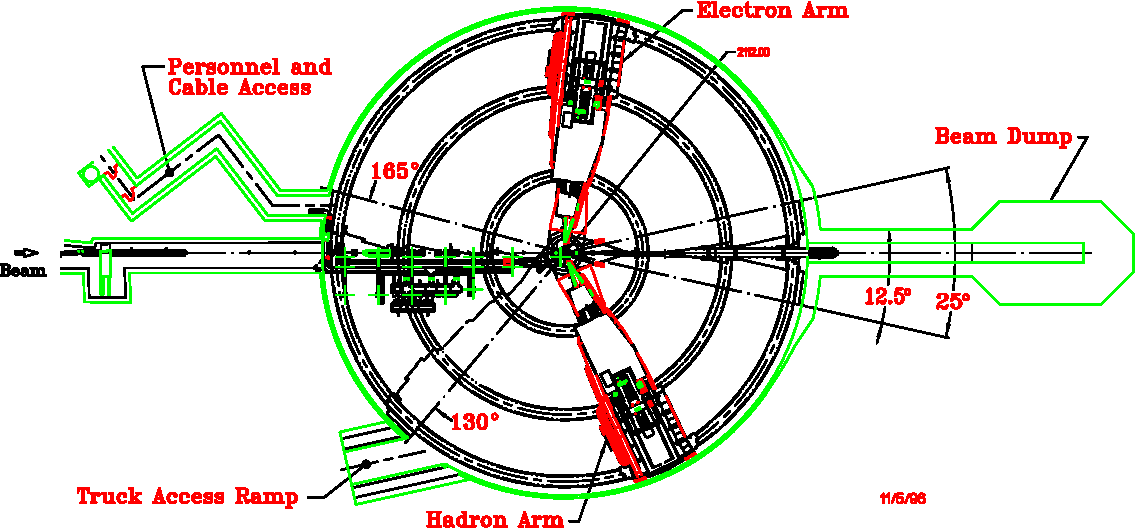
\includegraphics[angle=0,width=0.9\textwidth,clip]{figure0102_r}
\caption[Spectrometers: Plan View of Hall~A]{A bird's eye view of the Hall~A
end-station at TJNAF.}  
\label{fig:hrs_pv}
\end{center}
\end{figure}


A layout of the 4 GeV/c High Resolution Electron Spectrometer is shown 
on Figures~\ref{fig:hrs_pv} and \ref{fig:hrs_ev}.
Its main design characteristics are 
given in the attached table.  The spectrometer has a vertical bending 
plane and 45$^{\circ}$ bending angle.  The QQDQ design includes four 
independent superconducting magnets, three current-dominated 
cos2$\theta $ quadrupoles and one iron-dominated dipole with 
superconducting racetrack coils.  The second and third quadrupoles of 
each spectrometer have sufficiently similar field requirements that they 
are of identical design and construction.  The overall optical length, 
from target to focal plane, is 23.4 m.  Optically, the HRHS 
is essentially identical to HRES. In fact the two spectrometers can be used 
interchangeably to detect either positively or negatively charged particles 
as needed by any particular experiment. They are now commonly refered to 
as ``The Left Arm'' and ``The Right Arms'' rather than ``Hadron'' and ``Electron'' 

The support structure includes all system elements which bear the weight 
of the various spectrometer components and preserve their spatial 
relationship as required for 45$^{\circ}$ vertical bending optics.

The alignment and positioning system includes all the elements which 
measure and adjust the spatial relationship.  The support structure 
consists of the fabricated steel components which support the magnets, 
detector, shield house and associated equipment.  It is composed of the 
box beam, which supports the outer elements in fixed relative position 
atop the dipole; the dipole support bracket, upon which the dipole rests on 
the jacks; the cradle, upon which the dipole rests through the vertical 
positioning system, VPS; and a portion of the shield house load through 
the inboard legs of the gantry; the gantry, which supports the shield 
house and the magnet power supplies; and the bogies, which support the 
cradle-gantry assembly and roll on the floor plates and provide the 
driving power to move the two spectrometer arms.

The detector package (described in detail in Chapter \ref{chap:hrs-det})
is supported on the box beam and is surrounded by 
the shield house.  It must perform two functions, tracking and particle 
identification, PID.  The most important capability of focusing 
spectrometers is measuring precisely the momenta and entrance 
orientations of the tracks.  Momentum resolution of 10$^{-4}$ is 
obtainable, consistent with the resolution of the incident beam.

The actual configuration of the detector package varies from experiment to
experiment. The description given here is only an example of what is possible.
\infolevone{
A particle traversing the detector stack 
(Figure~\ref{fig:hrs_electron_det}) encounters two sets of horizontally
mounted, vertical drift wire chambers (x,y) with two planes of 368
wires in each chamber. The track resolution is $\sim$ 100 $\mu$m.  
From the chamber information both 
positions and angles in the dispersive and transverse directions can be 
determined.  The information from these chambers is the principal input 
of the tracking algorithms.

The chambers are followed by a scintillator hodoscope plane designated S1. 
This plastic scintillator array provides the timing reference for 
the drift chambers, and is also used in trigger formation and in combination 
with a second hodoscope pair it can provide time of flight particle 
identification.  These scintillators can also be used to perform crude 
tracking.

The next element encountered by a particle is a gas threshold \Cherenkov{} 
detector.  This is used for particle identification.  This gas threshold \Cherenkov{} detector can be swapped 
against an Aerogel detector, with a similar function.

The second hodoscope plane, S2, is located directly behind the 
gas \Cherenkov{}.  Its function is essentially the same as that of S1.  
In the hadron spectrometer an option exists to have this hodoscope 
pair be preceded by a third chamber, to improve tracking.
 Each of the two spectrometers 
have gas and Aerogel \Cherenkov{} detectors which can be used
 when they are in electron detection mode.

The final elements in the detector stack on HRSE are 
the pre-shower and the total-absorber lead glass shower 
calorimeter.  This is used for energy determination and PID.

\begin{figure}[tbp]
\begin{center}
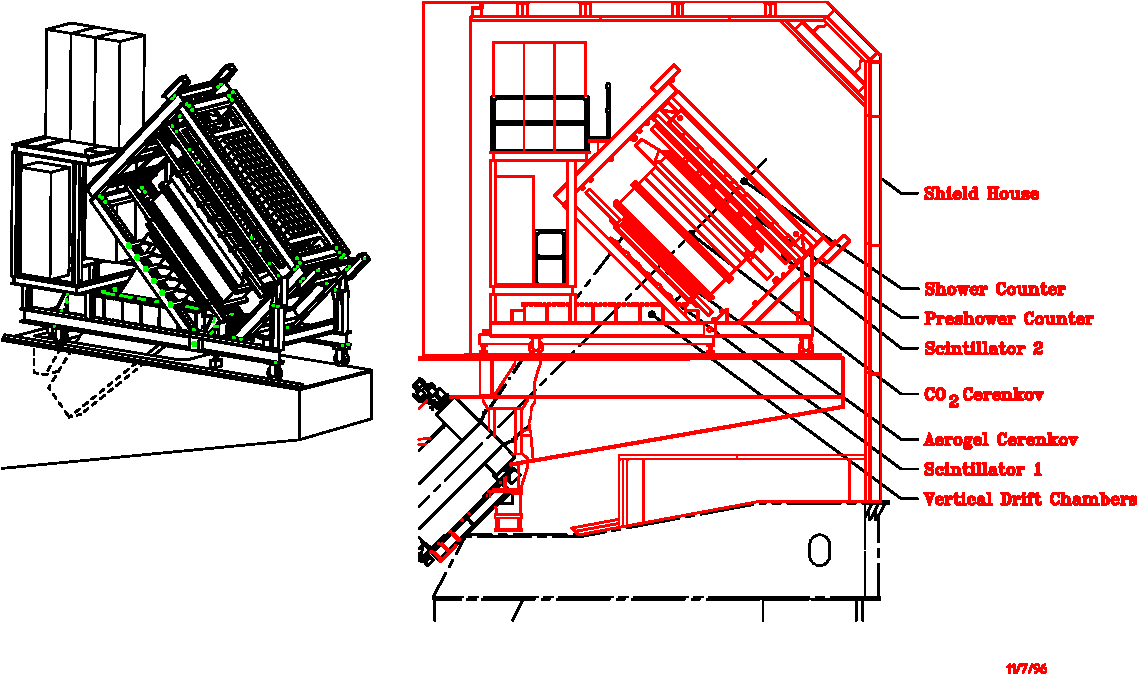
\includegraphics[angle=0,width=\textwidth,clip]{figure0103_r}
{\linespread{1.}
\caption[Spectrometers: Electron Arm Detectors]{The electron spectrometer detector stack.}
\label{fig:hrs_electron_det}}
\end{center}
\end{figure}

\begin{figure}[tbp]
\begin{center}
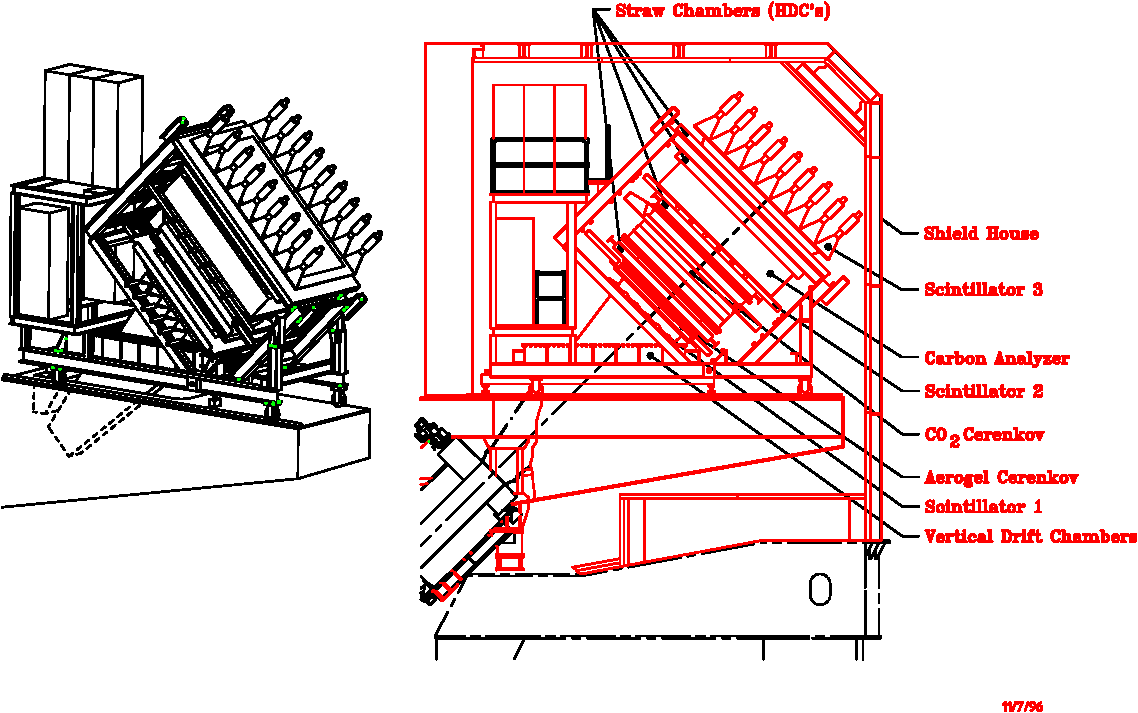
\includegraphics[angle=0,width=\textwidth,clip]{figure0104_r}
{\linespread{1.}
\caption[Spectrometers: Hadron Arm Detectors]{The hadron spectrometer detector stack.}
\label{fig:hrs_hadron_det}}
\end{center}
\end{figure}


The hadron detector is shown schematically in 
Figure~\ref{fig:hrs_hadron_det}.  It consists 
of two sets of (x,y) vertical drift wire chambers identical to those of the 
electron arm.  The remaining part of the detection system is used to 
define the level 1 trigger, as well as for particle identification and 
timing.  It consists of two minimally segmented planes of 
scintillation counters equipped with photomultipliers at both ends, and 
it includes \Cherenkov{} counters (gas CO$_2$ and Aerogel).

In addition, a proton polarimeter is installed in the back of the 
detector package to measure the polarization of the proton using a 
segmented carbon analyzer up to 60 cm in thickness to allow measurements 
over a wide range of proton energies.  A pair of front and a pair of 
rear straw tube wire chambers determine the incident and 
scattered angles, respectively.  The 
polarimeter detectors are dimensioned to accept a 20$^{\circ}$ cone of 
scattered protons.

Several support systems are necessary in addition to the basic 
components mentioned above.  They include gas supply systems for the 
wire chambers, high voltage supplies, readout electronics, a second 
level trigger, software for data analysis and testing, and a remotely 
controllable mechanical system.

For each spectrometer, all detectors are mounted on a 
single rigid support frame along with their associated electronics.  The trigger electronics are located on the support frame, next to the detectors.

} %infolev

To reduce the resolution degrading effects of multiple scattering, the 
entire interior of the spectrometer from the collimator box to the detector hut 
is a vacuum vessel.  The ends of this evacuated volume are capped by 
relatively thin vacuum windows.

\obsolete{
As mentioned, subsystems will be discussed in more detail in the next 
three sections.  The remainder of this section will describe some 
features common to the two spectrometers, then the following major 
sections will be devoted to the specifics that are not common.
} % obsolete

\begin{safetyen}{10}{15}
\section{Safety with Regards to the Spectrometer}
\label{sec:hrs-safety}
\end{safetyen}

The principle concern with the spectrometers is that they are large, 
and have associated vacuum, hydraulic, cryogenic and magnet systems all of 
which can be potentially dangerous.

The bogies which move the massive 1200 ton spectrometers must be 
carefully operated.  Inspection of the floor and wheels to ensure there is no 
debris which the wheels could ride over is mandatory.  Similarly 
personnel need to be aware that the spectrometers are moving so that no one 
inadvertently gets trapped.

The vacuum systems associated with the spectrometers are essentially 
pressure vessels (see Chapter \ref{chap:vacuum} for more details).
Care should be exercised so as not to puncture the 
windows.

The magnets themselves are installed inside cryostats.  These vessels 
are exposed to high pressures and are therefore equipped with safety 
relief valves and burst discs.

The hydraulic system originally intended to operate the vertical positioning system (VPS) 
and the horizontal positioning system (HPS) has effectively been dismantled, after problems were encountered during the initial attempted operation of the system.

The cryogenic system operates at elevated pressure at 4K.  One must 
guard against cold burns and take the normal precautions with pressure 
vessels when operating this system.  Only authorized personnel are permitted to install 
and take out U tubes.

The magnets have a great deal of stored energy as they are large 
inductors. Always make sure people are clear of them and that
the dump resistor is attached to the magnet.

There are several major safety concerns with regards to the detectors, 
namely 1) flammable gas located in the VDC, 2) ODH hazard due to 
CO$_2$ in the \Cherenkov{} counter, 3) high voltage due to the photo 
multipliers on the various detectors and 4) a thin vacuum window 
separating the detector array from the vacuum system in the 
spectrometers.

\infolevltone{
\begin{safetyen}{5}{10}
For more information consult the full OSP manual~\cite{HallAosp}.
\end{safetyen}
} %infolev

\begin{safetyen}{10}{15}
\subsection{Authorized Personnel}
\end{safetyen}

In the event that problems arise during 
operation of the magnets, qualified personnel should be notified
(see Table \ref{tab:hrs:personnel}).  
This includes any prolonged or serious problem with the source of magnet 
cryogens (the ESR).  On weekends and after hours there will be a 
designated individual on call for magnet services.  Any member of the 
Hall A technical staff is qualified to deal with unusual magnet 
situations but in the event of serious problems the technician on
call should be contacted.

\begin{namestab}{tab:hrs:personnel}{HRS: authorized personnel}{%
      HRS: authorized personnel. ''W.B'' stands for the white board 
      in the counting house.}
   \TechonCall{\em Contact}
   \EdFolts{}
   \JackSegal{}
   \HeidiFansler{}
   \JessieButler{}
   \AndrewLumanog{}
   \JasonGlorioso{}
   \MahlonLong{}
\end{namestab}

\infolevone{
\section{The Magnets of HRS}

Each HRS is composed of three superconducting quadrupole magnets, Q1, Q2, 
and Q3, and one superconducting dipole magnet.  The large quadrupoles were 
manufactured for JLab by SIEMENS, the small quadrupole by SACLAY, while 
the dipole was built for JLab by WANG NMR.  The quadrupole magnets are 
referred to as Q1, Q2, and Q3, where a particle first traverses Q1, then 
Q2 and the dipole magnet and finally traverses Q3.

The magnet system is followed by a large steel and concrete detector 
hut, in which all detector elements reside.  Most of the 
detector elements have been built by universities involved in the Hall A 
physics program.

The HRS magnet system is the cornerstone of the Hall A activities.  
Many of the experiments approved in Hall A center on physics at high 
resolution and other short-range phenomena, and rely on a spectrometer 
able to momentum analyze charged particles up to very high momenta.  The 
design value for the maximum momentum accessible to the HRS magnet 
system is 4 GeV/c.

\subsection{Magnets and Power Supplies}

The HRS magnet's are all superconducting and hence their coils must be 
maintained at cryogenic temperatures during operations.  The LHe 
required by the magnets is supplied by the End Station Refrigerator, ESR.

All the HRS magnets cryogenic services are supplied through the overhead 
cryogenic lines.  The distribution network begins at the distribution 
box over the pivot.  This box is connected to the rest of the network 
via the flexible transfer lines over the pivot.  The network is adjacent 
to the upstairs catwalk of the HRS.

Cryogenic information about each magnet is available on the control 
screens in the counting house, one for each magnet.  Normally during run 
periods the control screens are sent upstairs to the Hall A counting 
house and information on all the HRS magnets is available on the HRS 
control screen located in the center of the main console.  The control 
of all magnets is described in a following Section.

The power supplies for the magnets are located on the gantry balcony 
adjacent to the magnets.  The supplies are all cooled with low conductivity water (LCW).

\begin{safetyen}{10}{15}

Under no 
circumstances should any panel of any magnet power supply be opened by someone 
other than authorized personnel.  There are also 
signs posted listing the dangers of high magnetic fields.
\end{safetyen}

The control interface for the power supplies is available through the 
HRS control screen in the Hall A counting house.

\subsection{Quadrupole Magnets}

The quadrupoles provide some of the 
focusing properties of the spectrometer and to a large extent 
its acceptance.  Operating limits imposed on the 
quads are as follows: 1850A for Q2 and Q3 and 3250A 
for Q1.

All three quadrupoles for the HRS spectrometer are warm iron 
superconducting magnets.  The soft iron around the superconducting coil 
enhances the field at the coil center and reduces stray fields.  The 
basic parameters for the first quadrupole, Q1, are an effective length of about 
0.9 $m$, useful aperture of 0.3 $m$ and a field gradient of 9.5 
T/m.  To achieve the lowest possible angle setting of the HRS 
spectrometer (with respect to the beam line) the incident electron beam passes through
a notch in the outer yoke of Q1 when the spectrometer is at
its smallest angle of 12.5$^\circ$ . The 
other two quadrupoles, Q2 and Q3, are essentially identical with an 
effective (magnetic) length of about 1.8 meter, a useful aperture of 
0.6 $m$ and a field gradient of 3.5 T/m.
} %infolev

\infolevthree{
The maximum operating currents (assuming a 4 GeV/c momentum particle) 
for the quadrupoles are about 3000 A, 1700 A, and 1600 A, for Q1, Q2, and 
Q3, respectively.  This will render pole field values 
of 1.2, 1.0, and 1.0 T, respectively.  The energy stored in the 
quadrupole fields is sufficient to cause an unrecoverable quench if all 
the energy stored is dumped into the magnets.  Therefore a quench 
protection circuit is incorporated.  However, a quench can only happen 
if the cryomagnets have a helium level below the coil 60\% during operation.

The operating current to the Q1 quadrupole coils is provided by Danfysik 
System 8000 power supplies, which can operate up to 3500 A current and 5 
V.  The power supplies will be cooled with a combined maximum 
water flow of 45 liters per minute.

In addition to the main quadrupole windings, all quadrupoles have 
multipole windings.  To further optimize focusing properties of the HRS 
magnet system, it was intended to operate including some of these multipole 
trim coils in order to reduce higher order aberrations.
The operating current for these multipole corrections would be 
small, only (the multipole corrections are typically less than 2\% of 
the main quadrupole field), of order 50 A. Since the sextupoles were inadvertently 
installed rotated 90 $^\circ$ from their correct
orientation, these trim coils are now considered useless 
and there are at present no plans to use them.

\subsection{Cryogenic Procedures}

The cryogenics control is handled by the JLab Cryogenics Group.  The cryo control coordinator 
can be reached at the CHL (x7405) or by calling the MCC.

\subsection{First Time Startup Check List.}  

See attached check lists for all quadrupole and dipole magnets
 (Tables~\ref{tab:dip_check}, \ref{tab:q1_check}, and \ref{tab:q23_check}).
} %infolev

\infolevone{
\subsection{Dipole Magnet}

The dipole, by virtue of its field index, provides both
dispersion and focusing.  The present operations envelope 
states that the supply for the left HRS dipole may not be
operated at a current above 1800 A (4.4 GeV/c). The supply for the right HRS
dipole may not be operated above 1200 A (3.2 GeV/c), due to complications
caused by an internal short. 

The dipole for the HRS spectrometer is a superconducting, cryostable 
magnet.  Its basic parameters are an effective length of about 6.6 $m$, a 
bend radius of 8.4 $m$, and a gap width of 25 $cm$.  It is configured to 
achieve a 45 degree bending angle for 4 GeV/c momentum particles at a 
central field excitation of 1.6 T.  For the HRS dipole to reach 1.6 T 
an operating current of about 1500 A is required.
} %infolev

\infolevthree{
The dipole has been designed to achieve cryostability up to a field of 2 
T, and this property has been extensively tested up to a field of 1.6 T. 
 The cryostable coils are equipped with an energy removal circuit to 
cover the possibility of an unrecoverable quench.  However, this can 
only happen if the helium level drops below the coil during operation.  
The current to the coils will be provided by a Dynapower Corporation power 
supply, which can operate up to 2000 A and 10 V.  This 
power supply is located on the gantry beside the dipole, and will be 
cooled with a maximum water flow of 35 liters per minute.
The total water flow needed to cool the 4 power 
supplies for the HRS magnet system (dipole and quadrupoles) amounts to 
80 liters per minute, with a supply pressure of cooling water for Hall A 
of 100 psi.
} %infolev

\infolevtwo{
\section{Operation of the HRS Magnets}

\subsection{Introduction}

This is an abbreviated operating manual for 
the HRS superconducting magnets specifically designed for Hall A 
experimenters.  It provides instructions for setting currents, invoking 
NMR field regulation and general system monitoring.  Curious readers are 
directed to the references for more in-depth operating instructions and 
other technical manuals. Copies of the following supporting
documents are available in the Hall A Control Room and through the Hall A webpage
(see Table~\ref{tab:hrs-mag-manuals}).

\begin{table}[htp]
\begin{center}
\begin{tabular}{|l|l|}
\hline
References & \\
\hline 
WANG NMR Dipole & User Manual \\
Dynapower & Instruction Manual \\
Appendix & NMR Tesla meter \\
Appendix & NMR Field Regulation \\
Siemens/Fug & Q2/Q3 Magnet Instrumentation and Power Supplies \\
Saclay/Danfysik & Q1 Power Supply Manual \\
TOSP & HRS Dipole \\
TOSP & HRS Quadrupole Q1 \\
TOSP & HRS Quadrupole Q2, Q3 \\
HRS & SC Dipole Magnet Safety Review Vol. 2 \\
HRS & SC Quad Safety Review Vol. 1 \\ \hline
\end{tabular}
\end{center}
\caption[HRS Magnets: extra manuals]{HRS Magnets: extra manuals available in 
     Hall A Control Room.}
\label{tab:hrs-mag-manuals}
\end{table}

\subsection{Simple HRS Setting (Autopilot Mode)}
\label{sec:hrs-mag-set} 

 The magnets are controlled remotely using EPICS~\cite{EPICSwww} and
 EDM~\cite{EDMwww} GUI, provided that everything is working and power 
 supplies are turned on and ready to go.
 The appropriate interface runs
 on the computer \mycomp{hacsbc2} (see Section \ref{sec:contr-ha-menu}).
 On the ``Hall A General Tools'' control screen, in the upper left, there is 
 a rectangular box for each spectrometer (see Figure~\ref{fig:hrs_mag_cntrl}). 
\begin{figure}
\begin{center}
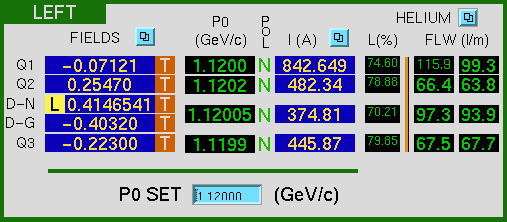
\includegraphics[angle=0,width=0.8\textwidth]{medm_halla_tools_1_cut1}
{\linespread{1.}
\caption[HRS: Magnets control]{A part of ``Hall A General Tools'' screen, 
        used for HRS (left) magnets control.}
\label{fig:hrs_mag_cntrl}}
\end{center}
\end{figure}

This box displays a brief summary of the status of the spectrometer
magnets and their cryogenic systems. The blue fields (with white
numbers) give readbacks of the magnetic fields and currents in each
magnet. The black fields also give readbacks, however in this case if
the text appears green those parameters are OK while if they are red
then that parameter is out of tolerance and may indicate a fault
condition. For example if the helium level goes below a certain point
the magnet will be automatically turned off.  In some cases it may be
desirable to monitor certain critical quantities on a strip chart
(e.g. magnet settings). A strip chart tool is available for this
purpose from the bottom of the ''EOS Menu'' button in the ''MyMenu'' window.

{\bf To set the spectrometers} for a given value of central momentum
(P0) type the desired P0 value into the light blue P0 SET box and hit
return. The magnets will be automatically 
set to the correct
values. All green numbers in the P0 column indicates that the desired
field or current settings have been reached. 

{\bf Caution:} Regarding the
dipoles, in general it's a bad idea to assume that at the first
instant that the P0 display turns green that the desired field has
been reached and you can start taking data. Stable field is in general
not achieved for from 15 to 30 minutes after reaching the nominal
desired field. This settling time depends on the magnet (the right dipole is
slower than the left dipole) and the magnitude of the field change (small
changes settle faster than big changes). Experimenters are advised to
observe both the field reading and current reading on the magnet in
question and verify that things are stable to their satisfaction
before proceeding.
 
\subsection{Powering Up Dipole Magnets:}

Use these instructions to recover from loss of a magnet due to a fault
(e.g. He level or lead flow fault). The order of actions matters. \\
(Contact Tech-On-Call if anything behaves funny or things don't
respond as expected. Sometimes after a trip an access to the Hall is
required to reset things).

\begin{list}{\arabic{enumi}.~}{\usecounter{enumi}\setlength{\itemsep}{-0.15cm}}
   \item Wait for Iout=0 (you can't and don't want to do anything while the magnet is in emergency fast dump mode.)
   \item While waiting, make a log entry re the fault. Give details such as time, coincident activities, and nature of the fault.
   \item Make sure the fault is cleared. (e.g. He level and flow rates returned to normal values and stable)
   \item In the HRS Right (Left) Dipole Systems' control panel:
   \begin{list}{}{\setlength{\itemsep}{-0.15cm}}
      \item[(a)] Press RESET (verify that all faults are cleared in the middle column)
      \item[(b)] Press ON (Display will indicate Power Supply ON and Magnet ENGAGED)
   \end{list}
\end{list}


Power supply and magnet are ready to go. From here you can return 
to "Autopilot Mode" (see Section \ref{sec:hrs-mag-set}).

\subsection{Starting Q1 Power Supply:}

 Do this when a fault causes the power supply to shut off.
 Wait for fault to clear (watch He levels). 
\begin{list}{\arabic{enumi}.~}{\usecounter{enumi}\setlength{\itemsep}{-0.15cm}}
   \item Push POWER OFF/RESET (check all faults cleared)
   \item Select desired polarity
   \item Push POWER ON
   \item Type in Setpoint (Amps) (light blue field) or re-enter P0 in Autopilot Mode.
\end{list}

\subsection{Starting Q2/3 Power Supply:}

 Do this when a fault causes the power supply to shut off.
 Wait for cause of fault to clear (watch He levels). 
 \begin{list}{\arabic{enumi}.~}{\usecounter{enumi}\setlength{\itemsep}{-0.15cm}}
   \item Push RESET 
   \item Select desired polarity
   \item Push ON
   \item Type in Current Set (light blue field) or re-enter P0 in Autopilot Mode.
\end{list}

} %infolev

